\chapter{算法设计和优化}

\section{InSAR 成像算法简介}

\subsection{InSAR 测高原理}

讨论并行 InSAR 成像算法之前,先对基本的算法原理做一个简单回顾。

\begin{figure}[ht]
\centering
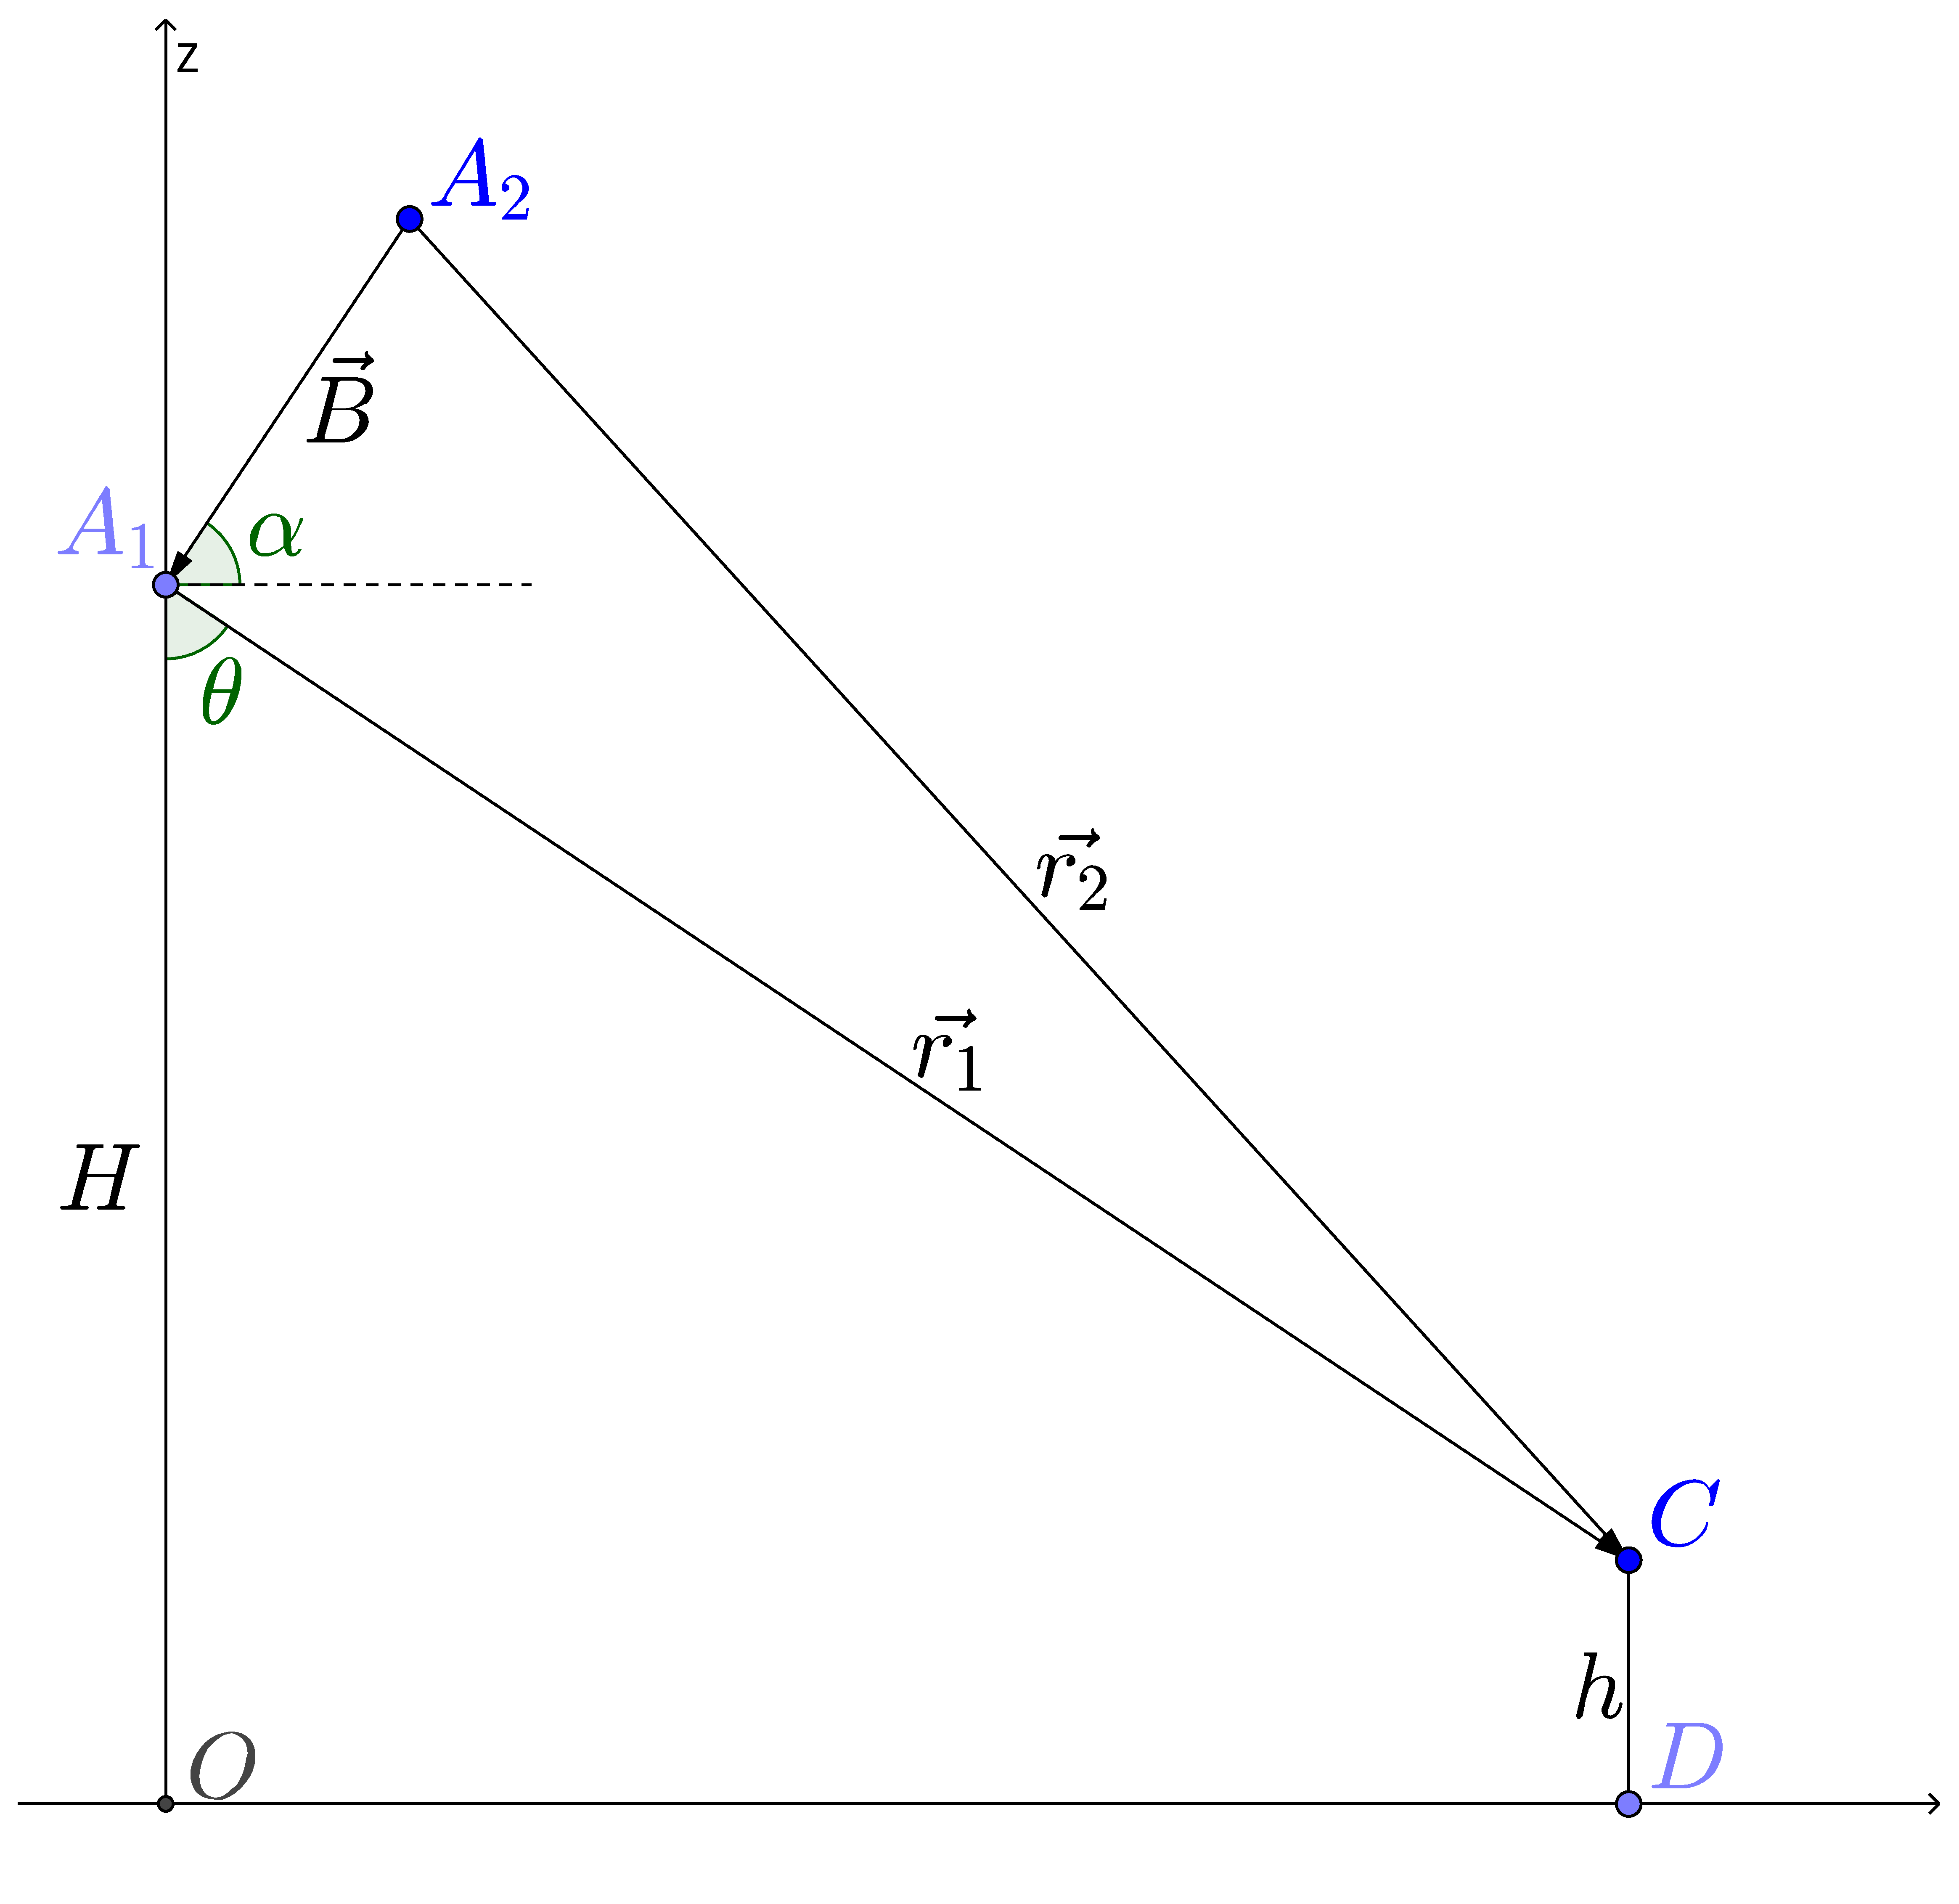
\includegraphics[width=0.4\textwidth]{insar_simple}
\caption{InSAR 高程测量基本原理} \label{fig:insar_simple}
\end{figure}

图 \ref{fig:insar_simple} 展示了利用两个 SAR 雷达观测同一地面单位进行 InSAR 测高的基本原理。InSAR 测量地表形变的原理与之类似。$A_1$ 和 $A_2$ 表示主天线和副天线位置,两天线空间位移矢量为 $\vec{B}$,称为 InSAR 基线,角度 $\alpha$ 为基线与水平面夹角。$C$ 为地面目标点,相对于两天线的位移矢量分别为 $\vec{r_1}$ 和 $\vec{r_2}$,称为斜距。角度 $\theta$ 为主天线观察方向与竖直方向的夹角,称为下视角。

斜距矢量 $ \vec{r_1} $ 和 $ \vec{r_2} $ 可以根据天线方向和微波信号双程旅行时得到;雷达位置或 SAR 卫星轨道,即基线 $\vec{B}$ 和天线高度 $H$,也可以认为是已知的。

由简单的几何关系可知,目标点高度可以表示为:

\begin{equation}
    h = H - r_1 \cos\theta
\end{equation}

为了得到 $\theta$,分别从主天线和副天线取得 SAR SLC 图像。目标点 $C$ 在两幅图像上的复像素值 $P_1$ 和 $P_2$ 可以表示为:

\begin{equation}
\begin{split}
    P_1(\vec{r_1}) = A_1(\vec{r_1}) \exp(i \frac{4\pi}{\lambda} r_1) \\
    P_2(\vec{r_2}) = A_2(\vec{r_2}) \exp(i \frac{4\pi}{\lambda} r_2) \\
\end{split}
\end{equation}

将两幅 SLC 图像共轭相乘,即得到一幅干涉图像:

\begin{equation}
    P_{\textrm{int}} = P_1^* P_2 =  A_1 A_2 \exp(i \frac{4\pi}{\lambda}(r_2 - r_1))
\end{equation}

干涉图相位项中的 $ r_2 - r_1 $ 可以通过余弦定理展开:
\begin{equation}
\begin{split}
    r_2 - r_1 &= r_1 (\frac{r_2}{r_1} - 1) \\
              &= r_1 \sqrt{1- \frac{\vec{r_1} \cdot \vec{B}}{r_1} + (\frac{B}{r_1})^2}
\end{split}
\end{equation}

基线长度 $B$ 一般远小于斜距 $r_1$、$r_2$,上式可以简化为:
\begin{equation}
    r_2 - r_1 = - \vec{r_1} \cdot \vec{B} = - r_1 B \cos(\frac{\pi}{2} - \theta + \alpha)
\end{equation}

故 $\theta$ 可以通过干涉图相位求出,进而得到目标点高程 $h$。然而,实际上回波相位(SAR 图像相位)是折叠到一个 $2\pi$ 周期内的,因此干涉图相位的值域也折叠在一个 $2\pi$ 周期中,这称为相位缠绕(phase wrap)。连续的相位值仍可以通过一些相位解缠算法估计出来。

实际使用 InSAR 测高时,还必须考虑地球曲率的影响。测量地表形变或位移时,原始地形引起的相位差也要通过数字高程模型去除。在过去,雷达轨道信息的精度也会影响 InSAR 成像精度;近些年,得益于卫星定位技术的发展,雷达轨道已经可以比较精确地获知。此外,电离层噪声、对流层噪声等因素也会影响 InSAR 成像的精度。

\subsection{InSAR 成像算法}

虽然 InSAR 测高原理非常简单,但实际的成像算法要复杂得多。主要可以归纳为以下若干步骤:

\textbf{SAR 成像和预处理}:相位差的测量精度决定了 InSAR 测高的精度。进行干涉的两幅 SAR 图像必须对成像区域有较好的聚焦,并且具有合适的基线长度,往往需要在若干组 SAR 数据中进行\textbf{筛选}。为了提取成像区域的有效信息,往往需要对 SAR 数据或者 SLC 图像进行\textbf{拼接}和\textbf{切割}。

\textbf{图像配准}:进行干涉成像之前,要通过图像配准将两幅 SAR 图像的像素精确对齐。SAR 图像像素大致对应于 SAR 雷达分辨率(数十米量级\cite{sandwell2011gmtsar})。虽然轨道数据已经可以较为精确地提供主副 SAR SLC 图像之间的偏移信息,但往往仍存在几个像素的误差。\citet{sandwell2011gmtsar} 指出,基于大地定位系统的卫星轨道数据在方位向的精度大约为1个像素、在距离向大约为2个像素。为了取得次像素级的配准精度,往往需要使用两幅图像的互相关特征进行修正。图像配准是成像程序中计算复杂度较高的一个步骤。

\textbf{干涉成像}:将对齐的主副 SAR SLC 图像进行共轭相乘,得到干涉图像。干涉图的相位被折叠到一个 $2\pi$ 周期上。根据上一节的推导,干涉图的相位信息反映了地面高程或地表位移信息。

\textbf{相位修正}:根据研究对象的不同,从干涉图中可选地去除地形相位、电离层延迟等不需要的相位项,以及滤除各种影响结果精度的噪声。

\textbf{相位解缠}:利用(一般情况下)高程或形变的连续性,从折叠相位恢复出连续变化的相位,以在较大的尺度上反映高程或形变信息。

上述步骤即为 InSAR 成像程序的主要功能。除此之外,包括 GMTSAR 在内的 InSAR 处理软件还支持地形图叠加等辅助分析功能,研究人员可以按需进一步处理。

\section{InSAR 成像算法 CPU 并行优化}

本节将以 GMTSAR 中图像拼接预处理和相位解缠两个程序模块为例子,介绍 CPU 并行的 InSAR 成像程序的算法设计和具体实现。

\subsection{并行图像配准算法设计}

GMTSAR 将主 SAR SLC 图像像素到副 SLC 图像之间的映射近似为一个二维仿射变换,可以通过6个变换参数定义。主 SLC 图像的像素 $(x_i, y_i)$ 因为轨道偏移被映射到副 SLC 图像上的 $(x_i', y_i')$,两个坐标通过仿射变换矩阵相联系:

\begin{equation}
\begin{bmatrix}
  t_i x_i' \\
  t_i y_i' \\
  t_i \\
\end{bmatrix}
= \begin{bmatrix}
       a & b & c \\
       d & e & f \\
       0 & 0 & 1 \\
\end{bmatrix}
\begin{bmatrix}
  x \\
  y \\
  1 \\
\end{bmatrix}
\end{equation}




\subsection{并行图像拼接算法设计}

\subsection{其他程序模块的并行优化}
